\subsection{時制の持つ意味}

\begin{figure}[h]
  \centering
  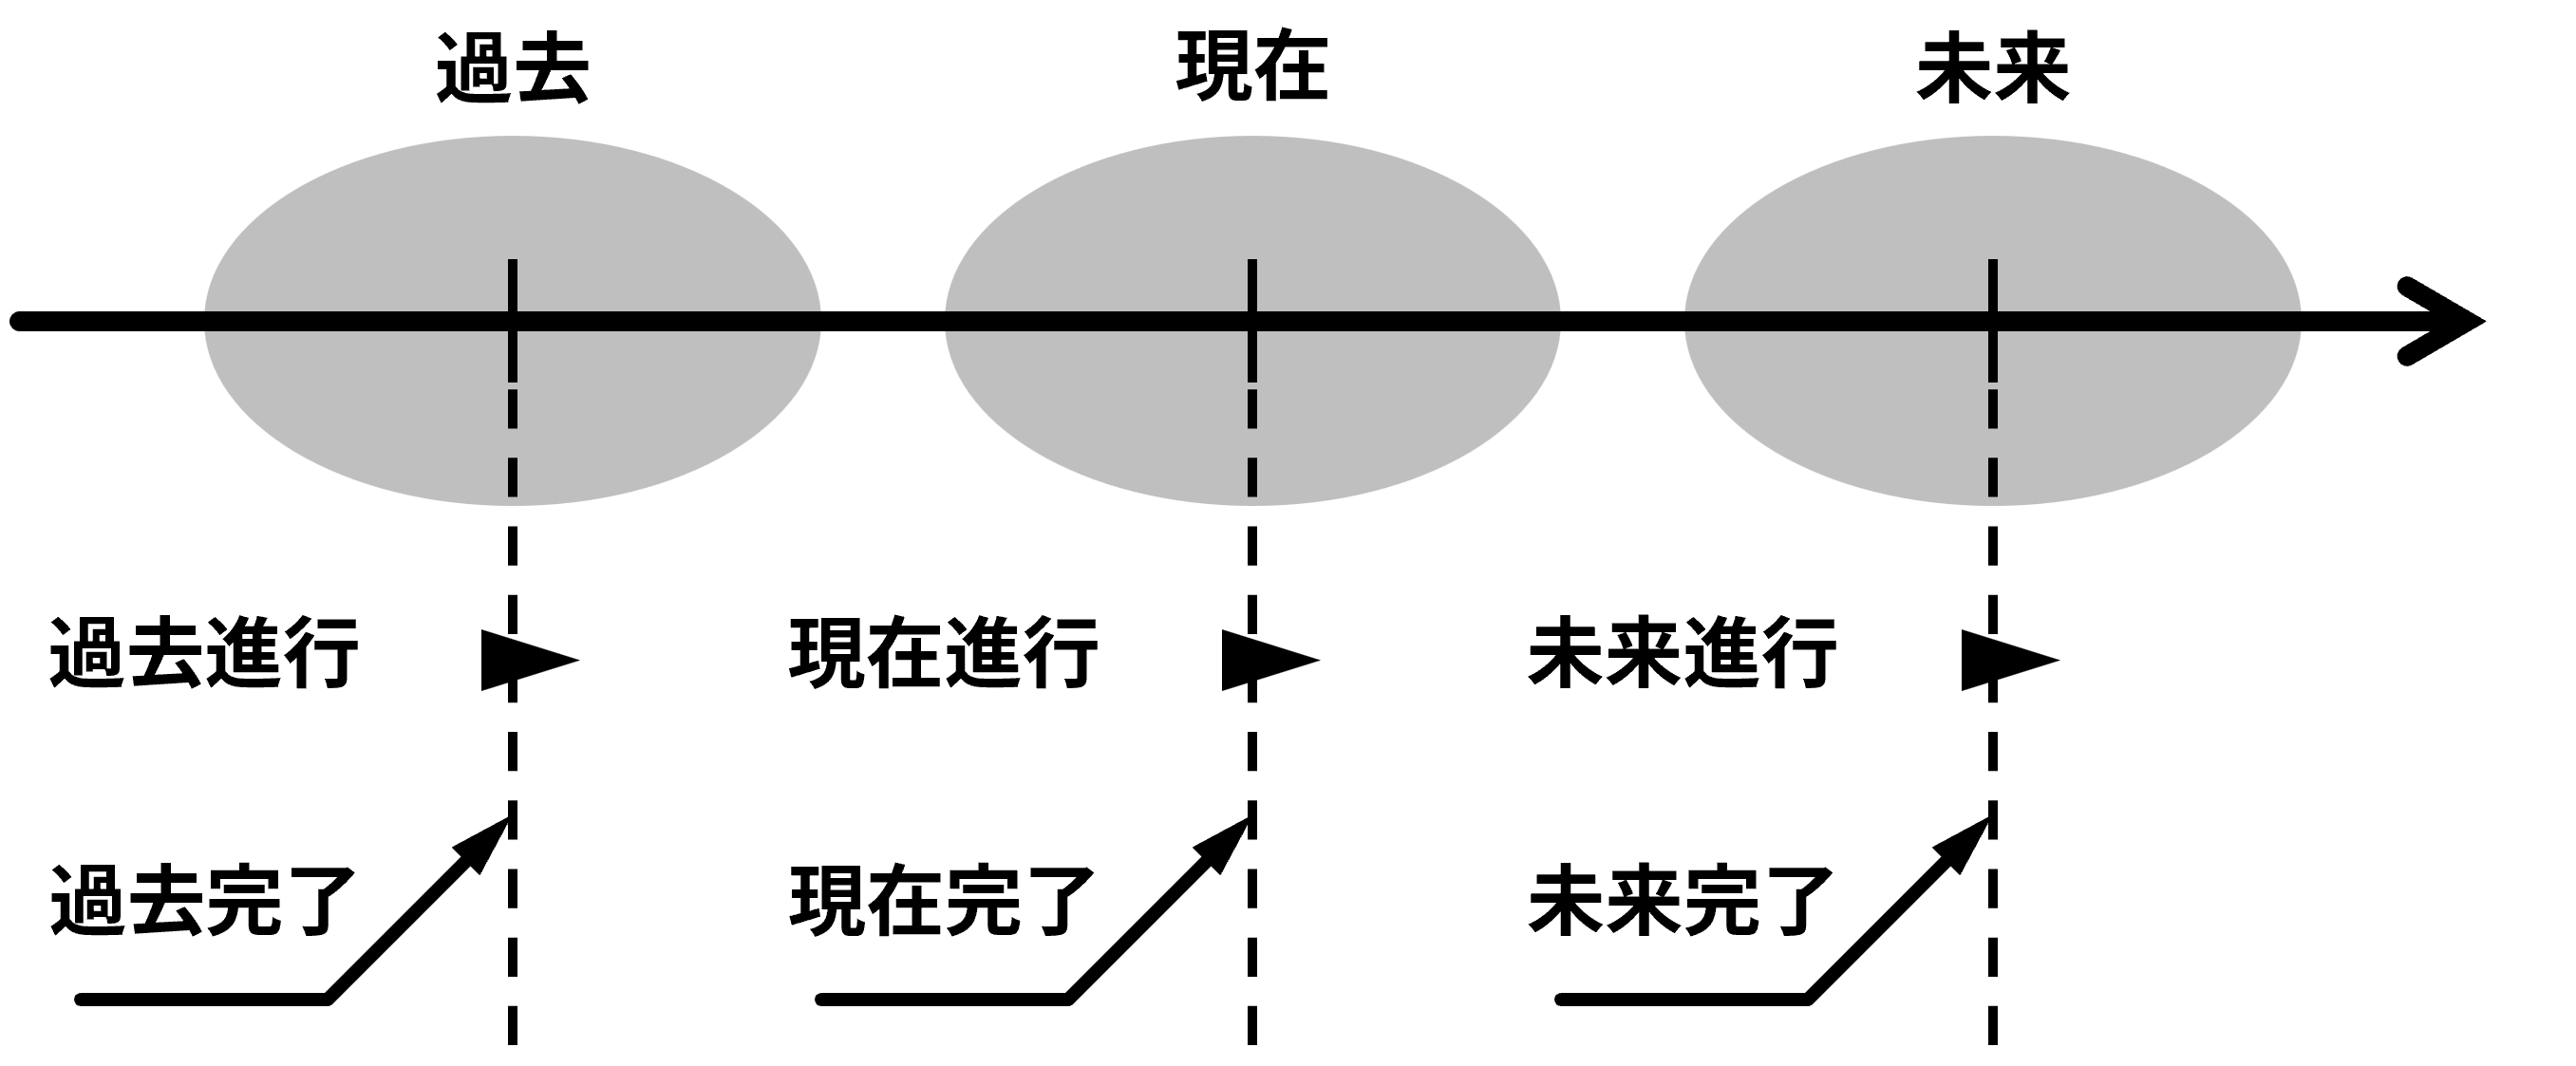
\includegraphics[width=100mm]{fig01.png}
\end{figure}

\subsubsection{現在・過去・未来}

単純な現在は、ざっくりと現在の時点付近のことを述べるのに使う。また、習慣などの反復的な行いや、普遍的な事実について述べるときにも使う。

単純な過去と未来についても、ざっくりとある過去の時点やある未来の時点付近のことを述べるのに使う。

\subsubsection{進行}

進行形は、ある時点で何かの動作や状態が継続しているときに使う。
現在進行形は自明に現在時点についての話だと自明にわかるが、過去進行形と未来進行形はどの時点で進行中なのかを特定させる必要がある。
たとえば、以下の例文を考える。

\begin{align}
  &I ~ am ~ playing ~ the ~ piano \text{.}\\
  &I ~ was ~ playing ~ the ~ piano ~ when ~ my ~ father ~ came ~ home \text{.}\\
  &I ~ will ~ be ~ playing ~ the ~ piano ~ when ~ my ~ father ~ comes ~ home ~ tomorrow \text{.}
\end{align}

どちらも「私はピアノを弾いている最中」であるという文章であるが、一つ目は現在進行形である一方で、二つ目は過去進行形、三つ目は未来進行形である。
後ろの二つでは「どのときに」ピアノを弾いている最中だったのかを示す必要があるため、「父が帰ってきたとき」「明日父が帰ってくるとき」というように過去や未来のどの時点かを特定する文言が入っている。
他にも「昨日の何時」などのように時間を指定する文言が入ることがある。
一方で、単に「昨日」や「先週」というような時間的に幅のある文言が入ることはない。
ちなみに、三つ目のwhen節について、「〇〇するとき」という副詞節のwhen節の中では、たとえ未来のことであっても未来形を使うことができない。
よって、単に現在形での表現になっている。

\subsubsection{完了}

完了には、完了結果・経験・継続の三つの使われ方がある。
どれにも共通していることとしては、「ある時点から見たときの、過去からある時点までの時間の流れ」に着目している点である。
また進行形と同様に、現在完了は現在までについての話だと自明にわかるが、過去完了や未来完了はどの時点までの話なのかを特定させる必要がある。

\paragraph{完了結果}\quad\\

完了結果は、「ある時点でVし終えた」という意味である。

\begin{align}
  &I ~ have ~ finished ~ my ~ homework \text{.}\\
  &I ~ had  ~ finished ~ my ~ homework ~ by ~ dinner ~ yesterday \text{.}\\
  &I ~ will ~ have ~ finished ~ my ~ homework ~ by ~ dinner ~ tomorrow \text{.}
\end{align}

一つ目の文章なら「現時点で」、二つ目と三つ目の文章なら「昨日(明日)の夕食までに」宿題を終わらせているという文章になる。
特に、「ちょうどVした」という意味の$just$、「既にVした」という意味の$already$、「まだVしていない」という意味の$not \sim yet$などと共に使われることが多い。



\subsection{各時制の表し方}

それでは、動詞の活用をおさえたうえで、時制について学ぶ。
時制とは、その文章がどの時点での動作・状態を表すのかというものであり、動詞を活用させたり助動詞を挿入することでそれを表す。

\subsubsection{現在・過去・未来}

\begin{itemize}
  \item 過去\\
  動詞を過去形(Vp)にする。\\
  助動詞がある場合は助動詞を過去形にして動詞を原形に戻す。
  \item 現在\\
  動詞を現在形にする。\\
  助動詞がある場合は助動詞を現在形にして動詞を原形に戻す。\\
  三単現の場合は動詞を三単現の形に活用する。\\
  助動詞がある場合は助動詞を三単現の形に活用して動詞を原形に戻す。\\
  (ただし、三単現の活用がある助動詞は$do \rightarrow does$のみなので、ほとんど考える必要はない)
  \item 未来\\
  助動詞willを挿入する。
\end{itemize}

\subsubsection{進行・完了}

\begin{itemize}
  \item 進行\\
  まず動詞を現在分詞(Ving)に変化させる。\\
  ただ、そうなると活用によって動詞が形容詞となるので、文から動詞がなくなる。\\
  そこで、現在分詞の直前に動詞としてbe動詞を挿入する。\\
  \begin{equation}
    V \rightarrow be + Ving
  \end{equation}
  \item 完了\\
  まず動詞を過去分詞(Vpp)に変化させる。\\
  ただ、そうなると活用によって動詞が形容詞となるので、文から動詞がなくなる。\\
  そこで、現在分詞の直前に動詞としてhaveを挿入する。\\
  \begin{equation}
    V \rightarrow have + Vpp
  \end{equation}
  \item 完了進行\\
  完了と進行の合わせ技をする。\\
  進行形への変化をしてから完了形への変化をすることで完了進行形となる。\\
  \begin{align}
    \begin{aligned}
      V & \rightarrow be + Ving\\
        & \rightarrow have + been + Ving
    \end{aligned}
  \end{align}
\end{itemize}

\subsubsection{複合時制}

現在・過去・未来の3種類と、単純(進行でも完了でもない普通の時制)・進行・完了・完了進行の4種類で、$3 \times 4 = 12$種類の時制が存在する。
それぞれの変形がどのようになるかを以下の表でまとめる。

\begin{table}[h]
  \centering
  \begin{tabular}{clll}
    \hline
     & \multicolumn{1}{c}{過去} & \multicolumn{1}{c}{現在} & \multicolumn{1}{c}{未来}\\
    \hline \hline
    単純 & Vp & V & will V\\
    進行 & be(was/were) Ving & be(is/am/are) Ving & will be Ving\\
    完了 & had Vpp & have Vpp & will have Vpp\\
    完了進行 & had been Ving & have been Ving & will have been Ving\\
    \hline
  \end{tabular}
\end{table}

\subsubsection{文法上の注意点}

ここまで読んで教えてもらった知識と違うと感じる人もいるだろう。
学校教育でもインターネット上の情報でも、はたまた歴史ある辞書でも、完了形のhaveは助動詞として紹介されているからだ。
その代わりに、過去分詞になった動詞を準動詞と呼び動詞として働くものとしている。
これは、意味上の動詞を動詞として扱いたいという考えのもと作られたメソッドである。
当たり前だが、完了形だろうが進行形だろうが意味上の動詞はVのまま変化しない。
だから、過去分詞になったとしてもVppを動詞ライクなものとして扱いたいのだ。
しかし、ここでは分詞になったらもはや動詞ではなくなるという考えのほうを重視し、形式上の動詞としてhaveを置くことにした。
もちろん、この考えにもデメリットがある(後述の疑問形の作り方の部分に影響する)ので、どちらの発想も頭に入れておくに越したことはない。
ややこしい話なので、一旦は「とりあえず完了のhaveは動詞として考えるけど、助動詞的な役割をすることもあるんだな」と思っておいてもらえるとありがたい。


